\documentclass{article}
\usepackage[]{graphicx}
\usepackage[]{xcolor}
\usepackage{alltt}
\usepackage[left=2.3cm,right=2.8cm, top = 2.2cm, bottom = 3cm]{geometry}
\usepackage{amsmath}
\usepackage{amssymb}
\usepackage{natbib}
\PassOptionsToPackage{hyphens}{url}
\usepackage{url}
\usepackage[disable]{todonotes}
\usepackage{multicol}
\usepackage{rotating}
\usepackage{booktabs}
\usepackage[colorlinks=false]{hyperref} 
\urlstyle{same}
\usepackage{lineno}
\linenumbers


% to handle authorship footnotes as numbers:
\makeatletter
\let\@fnsymbol\@arabic
\makeatother

\newcommand{\ra}[1]{\renewcommand{\arraystretch}{#1}}
\newcommand{\changed}[1]{#1}


\begin{document}


\title{To log or not to log}
  \author{Anonymous Alpaca\thanks{All Alpaca friends} $^{,}$\thanks{The Zoo} $^{ , *}$}

\maketitle

\begin{abstract}
In the abstract, this article is a very good one. 
\end{abstract}

\bigskip

{\footnotesize $^*$ Correspondence to: Anonymous Alpaca (\url{anonymous@alpaca.com}))}



\newpage

% General thought: maybe easier to do with WIS rather than CRPS? 
% Could do WIS in the main paper and CRPS in the SI? 

% We could look at the log growth rate
% with any linear model, an additive effect on the log growth rate would mean a multiplicative effect on the growth rate

\section{Introduction}

\paragraph{Role of forecasts and problem in comparing them}

Forecasts play an important role in decision-making in many areas such as for example economics [Citations], agriculture [Citations] and epidemiology [Citations]. Forecasts are most useful if they are probabilistic in nature [Citation e.g. Held et al.], meaning that in addition to a point prediction, forecasters also provide a predictive distribution to quantify their uncertainty. Through the COVID-19 pandemic forecasts of case numbers, hospitalisations and deaths have had a strong influence on public policy and there merits and limitations have been widely discussed by politicians, experts and laypeople alike. Probabilistic COVID-19 Forecasts from different research institutions have been systematically collected and aggregated by the US Forecast Hub [Citation], the German and Polish Forecast Hub [Citation] and the European Forecast Hub [Citation]. One major challenge in comparing and evaluating these forecasts is that it is not immediately how to deal with targets on different orders of magnitudes (e.g. case numbers and hospitalisations) or how to take the exponential nature of epidemiological processes into account. In this paper we will argue that evaluating forecasts on a logarithmic, rather than a natural scale, may help alleviate some of these concerns and may be better suited to epidemiological forecasts. 

%Forecasts should be well calibrated (i.e. should not systematically deviate from the observations) and subject to calibration should be as precise as possible (Cite Gneiting). 

\paragraph{Context / explanation of scoring rules}
Generally, probabilistic forecasts like those submitted to the Forecast Hubs are usually evaluated using proper scoring rules [Cite Gneiting et al. 2007]. A proper scoring rule incentivises any forecaster to state their true best belief and on average always gives the best score to the forecaster who reports a predictive distribution that is equal to the data-generating distribution. Forecasts submitted to the Forecast Hubs were required to follow a quantile-based format where forecasters would report a set of 23 quantiles (11 symmetric prediction intervals as well as a median prediction). A natural choice for quantile-based forecasts is the (weighted) interval score (WIS) [Cite Bracher et al.]. 

The WIS (lower values are better) can be decomposed into a dispersion component and penalties for over- and under-prediction. For a single prediction interval, the interval score is computed as 
\begin{equation}
 IS_\alpha(F,y) = (u-l) + \frac{2}{\alpha} \cdot (l-y) \cdot 1(y \leq l) + \frac{2}{\alpha} \cdot (y-u) \cdot 1(y \geq u),    
\end{equation}

where $1()$ is the indicator function, $y$ is the observed value, and $l$ and $u$ are the $\frac{\alpha}{2}$ and $1 - \frac{\alpha}{2}$ quantiles of the predictive distribution $F$, i.e. the lower and upper bound of a single central prediction interval. For a set of $K$ prediction intervals and the median $m$, the WIS is computed as a weighted sum, 
\begin{equation}
WIS = \frac{1}{K + 0.5} \cdot (w_0 \cdot |y - m| + \sum_{k = 1}^{K} w_k \cdot IS_{\alpha}(F, y)),    
\end{equation} 
where $w_k$ is a weight for every interval. Usually, $w_k = \frac{\alpha_k}{2}$ and $w_0 = 0.5$

The WIS is closely related to the continuous ranked probability score (CRPS, lower values are better) [Cite Gneiting 2007], which itself can be understood as a generalisation of the absolute error to probabilistic forecasts. For an increasing set of equally-spaced prediction intervals the WIS converges to the CRPS and shares many of its properties. The CRPS measures the 'distance' of the predictive distribution to the observed data-generating distribution as 



\begin{equation}
    \text{CRPS}(F, y) = \int_{-\infty}^\infty \left( F(x) - 1(x \geq y) \right)^2 dx,
\end{equation}

where y is the true observed value and F the CDF of predictive distribution. Often the following alternative representation is used
\begin{equation}
    \text{CRPS}(F, y) = \frac{1}{2} \mathbb{E}_{F} |X - X'| - \mathbb{E}_P |X - y|,
\end{equation}
  
where $X$ and $X'$ are independent realisations from the predictive distributions $F$ with finite first moment and $y$ is the true value. In this representation we can simply replace $X$ and $X'$ by samples sum over all possible combinations to obtain the CRPS.  

Another proper scoring rule commonly used is the log score [CITATION], which we will not discuss further in this paper.  

\paragraph{Problems with the WIS and CRPS in an epidemiological setting}
Their relation to the absolute error means that both the CRPS and the WIS scale with the prediction target. Forecasts of COVID-19 cases, for example typically have much higher scores than forecasts of hospitalisations of death. Similarly, when looking at performance across different locations or over time, average scores will be dominated by locations and times with high incidences. Single outliers also can have a disproportionate effect on aggregate scores. One can argue that this is meaningful and that we should care most about places and periods when incidences are high (maybe cite Bracher et al.). However, this may not always be true and is clearly not desirable when comparing performance of a model on different prediction targets: case numbers are not necessarily more important than hospitalisations, just because observed values tend be an order of magnitude higher. This makes forecasts often hard or impossible to compare. Distributions of forecast scores are usually highly skewed making it hard to model them using standard linear models. Researchers instead often resorted to evaluating different prediction targets or locations completely independently, a process that is often cumbersome and makes it hard to identify factors that systematically affect scores. In any epidemiological setting there is also a noticeable tension when processes (such as the spread of a disease) that are usually modelled multiplicatively are scored in terms of absolute (additive) errors. 

\paragraph{Outline of what we do} 
A natural proposition is therefore to score forecasts on a logarithmic scale, making it easier to model and compare scores across targets by alleviating concerns about skewed forecast scores and also taking into account the multiplicative nature of epidemiological processes. In this paper we will ...

%\begin{enumerate}
%    \item Effects / Interpretation of scoring on a log scale
%    \item Appropriate scales for epidemiological (and possibly other) processes
%    \item Modelling log scores
%\end{enumerate}



%%%%%%%%%%%%%%%%%%%%%%%%%%%%%%%%%%%%%%%%%%%%%%%%%%%%%%%%%%%%%%%%%%%%%%%%%%%%
\section{Scoring on a log scale}

\paragraph{What we propose}
Proper scoring rules yield a score as a function of a forecast $x$ and a corresponding observation $y$. For epidemiological forecasts of positive quantities we propose to replace WIS and CRPS scores on the natural scale computed as 
%
\begin{equation}
S(x, y),     
\end{equation}
%
by scores computed on the logarithmic scale as 
%
\begin{equation}
S(\log{(x + 1)}, \log{(y + 1)}),    
\end{equation}
%
where $S()$ is either the WIS or the CRPS and one is added to deal with zeros in the data. The so computed score is still proper, as for a single forecast the order between different forecasters is not affected by the monotone transformation. Differences in the ranking between forecasters only appear when averaging over multiple forecasts, as deviations from the perfect forecast get penalised differently depending on whether forecasts are scored on the log or the natural scale. Note that simply taking the log of a score computed on the natural scale, i.e. computing $\log S(x, y)$ results in an improper score and is therefore not advised. We illustrate this point in Figure \ref{fig:log-improper} in the SI. 

\paragraph{Scoring the log means scoring the growth rate} Computing a score based on the logarithm of the forecast and the observation is approximately equivalent to scoring a forecast of a multiplicative growth rate of the forecast target. The growth rate is defined as 
%
\begin{equation}
    g_{t, t+1} = \frac{y_{t+1} - y_t}{y_t},
\end{equation}
%
where $y_{t+1}$ is the forecast target (e.g. reported cases of COVID-19), $y_t$ is the last known observation and $g_{t, t+1}$ is the growth rate between now ($t$) and $t+1$. This can be rewritten as 
%
\begin{equation}
y_{t+1} = (1 + g_{t, t+1}) \cdot y_t.
\end{equation}
%
If we score $\log y_{t_+1}$ rather than $y_{t+1}$, this changes to 
%
\begin{equation}
\log y_{t+1} = \log (1 + g_{t, t+1}) + \log y_t.    
\end{equation}
%
Note that $\log y_t$ is a known quantity that can be removed from both sides without changing the score. What is uncertain is $\log y_{t+1} - \log y_t = \log (1 + g_{t, t+1})$.  For small values of $g$, we lastly have 
\begin{equation}
    \log (1+ g_{t, t+1}) \approx g_{t, t+1}.
\end{equation}
%
When we score a forecast for $y_{t+1}$ on the log scale, the interval score for a single prediction interval changes as follows
%
\begin{align}
    \text{IS}_\alpha(\log F, \log y) = &(\log u - \log l) \\ 
    &+ \frac{2}{\alpha} \cdot (\log l - \log y) \cdot 1(\log y \leq \log l) \\
    &+ \frac{2}{\alpha} \cdot (\log y - \log u) \cdot 1(\log y \geq \log u).
\end{align}
%
Note that the values of the indicator functions stay the same as the logarithm is a monotonic transformation and the inequality is preserved. 
On the natural scale, $u$, $l$ are the lower and upper bounds of a central prediction interval for a forecast of $y_{t+1} = (1 + g_{t, t+1}) \cdot y_t$. 
We can rewrite these as 
\begin{equation}
   l = l^* \cdot y_t 
   \;\; \text{and} \;\; 
   u = u^* \cdot y_t,  
\end{equation}
where $u^*$ and $l^*$ are the lower and upper bounds of a prediction interval for $(1 + g_{t, t+1})$. Consequently, 
\begin{equation}
  \log l = \log l^* + \log y_t
  \;\; \text{and} \;\;
  \log u = \log u^* + \log y_t. 
\end{equation}
%
We can then rewrite the score for a forecast of $\log y_{t+1} = \log (1 + g_{t,t+1}) + \log y_t$ as
%
\begin{equation}
\begin{aligned}
IS_\alpha&(\log F_{t+1}, \log y_{t+a}) = \\
&((\log u^* + \log y_t) - (\log l^* + \log y_t)) \\
&+ \frac{2}{\alpha} \cdot ((\log l^* + \log y_t) - (\log (1 + g_{t, t+1}) + \log y_t)) 
     \cdot 1((\log (1 + g_{t, t+1}) + \log y_t) \leq (\log l^* + \log y_t) \\
&+ \frac{2}{\alpha} \cdot ((\log (1 + g_{t, t+1}) + \log y_t) - (\log u^* + \log y_t)) 
      \cdot 1((\log (1 + g_{t, t+1}) + \log y_t) \geq (\log u^* + \log y_t),
\end{aligned}
\end{equation}
%
which simplifies to 
%
\begin{equation}
\begin{aligned}
\label{eqn:is-log}
\text{IS}_\alpha(\log F_{t+1}, \log y_{t+a}) = &(\log u^* - \log l^*) \\
&+ \frac{2}{\alpha} \cdot (\log l^* - \log (1 + g_{t, t+1}) 
     \cdot 1(\log (1 + g_{t, t+1}) \leq \log l^*) \\
&+ \frac{2}{\alpha} \cdot (\log (1 + g_{t, t+1}) - \log u^*) 
      \cdot 1(\log (1 + g_{t, t+1}) \geq \log u^*).
\end{aligned}
\end{equation}

The left-hand side of equation \ref{eqn:is-log} was left unchanged. From the right-hand side we can see that for a single prediction interval, scoring the log of a forecast ($\log F_{t+1}$) against the log observed value ($\log y_{t+1}$) is exactly equivalent to evaluating a forecast for $\log (1 + g_{t, t+1})$. With $\log (1 + g_{t, t+1} \approx g_{t, t+1}$, this is approximately a forecast for the growth rate for small values of $g_{t, t+1}$. 
Conveniently, the decomposition of the WIS into dispersion, over-prediction and under-prediction is preserved. The interpretation of the components has now changed in that they now approximately represent uncertainty, over-prediction, and under-prediction with the growth rate. 

\paragraph{Additive vs. multiplicative errors}
Of course the growth rate (and more generally the term $\log (1 + g_{t, t+1})$) would be linked multiplicatively to the observed value on the natural scale. Recall that the WIS is closely linked to the absolute error. On the natural scale, we were conceptually evaluating an absolute error of our forecast with regards to the true observed value. Simplified to the case of a point forecast $\hat{y}_{t+1}$ we could express this as measuring an absolute error $\varepsilon_{t+1}$ such that
%
\begin{equation}
    \hat{y}_{t+1} = y_{t+1} + \varepsilon_{t+1}. 
¸\end{equation}
In the case of scoring the log forecast, where we evaluate an absolute error on $\log (1 + g_{t, t+1})$, it makes more sense to understand the error $y_{t+1}$ as being a multiplicative error $\varepsilon^*_{t+1}$ so that
\begin{align}
    \hat{y}_{t+1} &= y_{t+1} \cdot \varepsilon^*_{t+1} \\
    &= y_{t} \cdot (1 + g_{t, t+1}) \cdot \varepsilon^*_{t+1},
\end{align}
%
which on the log scale becomes to 
\begin{align}
    \hat{y}_{t+1} = \log y_{t} + \log (1 + g_{t, t+1}) + \varepsilon^*_{t+1}. 
\end{align}

The log transformation therefore changes which types of errors (additive or multiplicative) are penalised. The WIS and CRPS computed on the natural scale penalise large absolute errors, regardless of whether the error is large in relative terms. Predicting 101,000 cases instead of the true 100,000 will be treated equally to predicting 2,000 hospitalisations, rather than the 1,000 observed. The WIS and CRPS based on log-transformed values however, penalise relative errors. Forecasting 101,000 rather than 100,000 cases will be treated equally to forecasting 2,020, rather than 2,000 hospitalisations. The score is relative and therefore less dependent on the scale of the forecast quantity, making it easier to compare (relative) performance across different forecast targets, periods and locations. 

\paragraph{Note on propriety and shifting the focus of the evaluation}
Applying the log transformation preservers propriety of the scoring rule. The task of the forecaster has not changed and in both scoring scenarios, forecasters are incentivised to report their best possible forecast. Any forecast that is made already implicitly contains a statement about the growth rate of a process as well as about the expected absolute order of magnitude of the target. By scoring based on the log transformed forecasts and observations, we merely choose to shift the attention towards evaluating the forecaster based on relative errors, rather than absolute numbers. 

\section{What happens when you average many scores}

THIS COULD INCLUDE JOHANNES EXAMPLE

COULD ALSO JUST MAKE A SIMULATION. 
YOU TAKE 1000 little counties, combine them to 20 states with different sizes. Then you plot 


This means the WIS and CRPS on the natural scale are dependent on the scale of the forecast target, because forecasting errors will typically be large for large quantities. 
However, note that large relative errors will likely more often occur with small quantities (e.g. predicting 9, rather than 3 deaths), potentially giving undue weight to small quantities. Whether or not more weight is given to smaller or larger forecast quantities depends on the exact relationship between the mean and the variance of the quantity of interest. If the variance grows slower than the mean, then scores will on average be larger for small quantities than for larger ones. In practice, this can be partly mitigated by restricting the analysis to forecast targets with with higher incidences. 
% the phrase "scores give a higher weight to a or b" could be made clearer: This is about a scenario where you average across different targets and the average score is influenced by outliers


%COMPARISON TO SCORING THE ACTUAL GROWTH RATE - just harder to do and achieves the same thing? No objections if someone wants to? Might actually be better if there are negative values involved? 

%What about other things like scoring the square root of the forecast?


%\begin{itemize}
%    \item discuss how equations change for CRPS
%    \item Optional: Discussion of parallels to point forecasts and the point that you're still incentivised to report the median\\
%    \item discuss that even if both scoring rules are proper, they still penalise different things %differently. How does that change incentives for the forecaster? 
%\end{itemize}

\paragraph{What happens to the WIS / CRPS when you log it?}
\begin{figure}[h!]
    \centering
    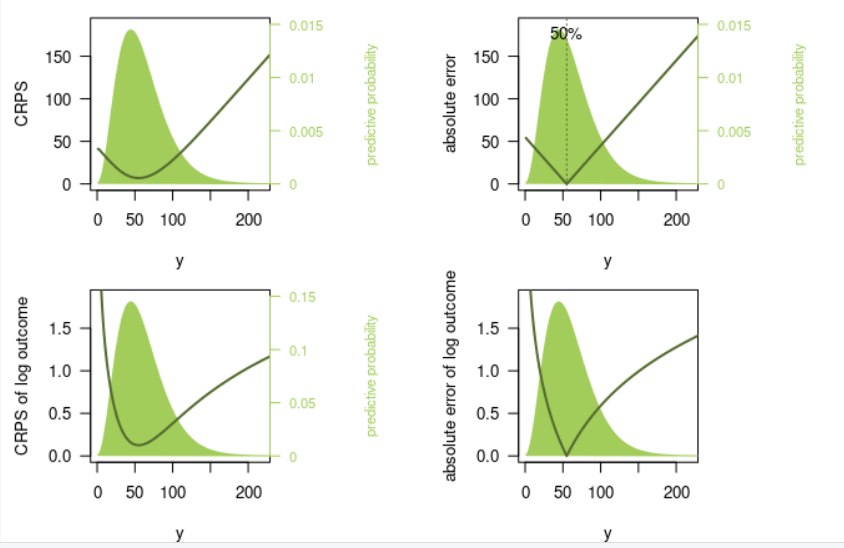
\includegraphics[width=0.9\textwidth]{output/crps log viz.png}
    \caption{Figure from Johannes: How CRPS changes when you log the observation}
    \label{fig:log-crps-viz}
\end{figure}



% could make an analysis re outliers: how do scores change if we remove the 1 or 2 worst forecasts? The one or two best forecasts?

\paragraph{detailed interpretation of plots and when you give larger scores to what}

\begin{figure}[h!]
    \centering
    
\includegraphics[width=0.9\textwidth]{output/placeholder-image.png}
    \caption{Plot that shows the scores for log and non log and how they change}
    \label{fig:change-in-scores}
\end{figure}

\paragraph{Option: empirical analysis} 
Score different things from the European / US Forecast Hub and plot the relationship between mean and variance. Plot log-scale scores for different things and see which of these influence average scores most \\
What happens to the decomposition of the WIS if we log? 



\section{Appropriate scales for epidemiological processes}
%Could also make this more general and compare any additive, multiplicative or even other processes and state which scale would be appropriate. 

\paragraph{Scoring epidemiological processes}
Epidemiological processes are generally multiplicative, others may be additive or even something else. We want to explore whether epidemiological processes should in principle be scored on a log scale. Also: are there any processes which shouldn't be scored on a log scale? 

\paragraph{What is the interpretation of logging in an epidemiological setting and is it appropriate?}

\paragraph{Over- and under-prediction}
If we want to keep this in, we could: 
\begin{itemize}
    \item Check whether there is actually a problem with over-prediction and under-prediction in the Hub. This could be the case because we are most interested in certain scenarios in which this might arise. 
    \item Discuss this in light of Johannes' analysis of how the decomposition of WIS values differs if the data are skewed
    \item compare this to the PIT-value-like relative bias scores we used for the German / Polish paper, which capture a relative tendency to over- or under-predict, rather than absolute penalties. 
\end{itemize}

\paragraph{Toy example: simulate an epidemic and apply 3 different models} Compare scores for these three models on the natural scale and the log scale

\paragraph{Optional: Empirical differences when going from natural to log-scale} 
We could score a lot of forecasts of the European Hub and show plots about how scores differs when going from natural to log-scale


\section{Modelling scores}
\paragraph{Motivation} Alternative is to use summary measures or pairwise comparison, which becomes cumbersome for many dimensions. 

\paragraph{caveats, practical limitations}
\begin{itemize}
    \item What kind of transformations can we do? Propose random effect models
    \item is there anything we can't do? 
    \item How does logging change the error distribution? On the natural scale, you have huge outliers. What's the appropriate error distribution to use? confidence intervals. Maybe we can only say something about the effects
\end{itemize}


\paragraph{Optional: Application to data from the Euro-Hub}
Also: what, empirically is the distribution of errors? 

\section{Other ideas}
\begin{itemize}
    \item Compare different predictive distributions and the score as a function of an outcome.
    \item ...
\end{itemize}




\section{Discussion}

\paragraph{summary of what we did}

\paragraph{context, implications, limitations}

\paragraph{outlook, future work}


 




\newpage

\appendix
\section{Supplementary information}

\begin{figure}[h!]
    \centering
    
\includegraphics[width=0.9\textwidth]{output/placeholder-image.png}
    \caption{Illustration of the fact that taking the log of WIS or CRPS results in an improper score}
    \label{fig:log-improper}
\end{figure}

\end{document}


%%%%%%%%%%%%%%%%%%%%%%%%%%%%%%%%%%%%%%%%%%%%%%%%%%%%%%%%%%%%%%%%%%%%%%%%%%%%
% Idea parking lot 
%%%%%%%%%%%%%%%%%%%%%%%%%%%%%%%%%%%%%%%%%%%%%%%%%%%%%%%%%%%%%%%%%%%%%%%%%%%%

%\begin{itemize}
%    \item idea of scores on logged data: interpretation as a measure of relative improvement, just as when you log the absolute error
%\end{itemize}

%\paragraph{What's there in the literature}

%\paragraph{Current problems / questions about scoring an epidemiological setting}
%probably narrow down to the ones we really want to discuss%
%There are limitations with what we can do with scores on a natural scale and open questions whether we can do these things on a log-scale and also whether a log-scale might be inherently more appropriate
%\begin{itemize}
    %\item Can't really model score on a natural scale as errors are heavily skewed. Is there a way to model scores to get insight about different factors that systematically influence scores
 %   \item make a plot somewhere that shows the distribution of scores
  %  \item Maybe epidemiological forecasts are inherently better suited to be scored on an absolute scale due to the multiplicative nature of processes (related to over-prediction > under-prediction)? Does the log-scale imply we are scoring the growth rate? 
   % \item unclear what trade-offs of logging / not logging are
    %\item what score (log, not log) matches closest what our intuition (or policymakers) think is good? 
    %\item are we better at forecasting deaths than cases? --> relative measure would help
    %\item There exists confusion about what can be done to a score in general (e.g. people want to take the median, which they shouldn't) %maybe don't add as an extra point
%\end{itemize}
